\chapter{Cloud-based Software}

The revolution of cloud-based software began with the combination of two aspects: \emph{powerful computer hardware} and \emph{high-speed networking}, which have led to the development of cloud computing, and \emph{virtualized resources} (e.g., compute, storage, platform) accessible on demand.

The main advantages of cloud-based software are:
\begin{itemize}
    \item \textbf{Scalability}: Maintains performance as load increases (useful when developers do not know the number of the product's customers).
    \item \textbf{Elasticity}: Adapts server configuration to changing demands (we want to avoid \emph{underprovisioning} and \emph{overprovisioning}).
    \item \textbf{Resilience}: Maintains service in the event of server failures.
    \item \textbf{Cost}: Most cloud services are \emph{pay-per-use} (no need to buy hardware).
\end{itemize}

\section{Virtualization and Containers}

As mentioned before, one of the main aspects that led to cloud-based software is \emph{virtualized resources}. When we refer to \emph{compute power}, we mean servers and many other devices. It is possible to host many virtual servers inside the same physical server, which utilize virtual machines.

The left stack of Figure \ref{fig:virtualizedresources} refers to a machine with an \emph{OS} and a \emph{Hypervisor} (which enables virtualization; the one shown in the figure is a Level 2 Hypervisor, which depends on the OS. The Level 1 Hypervisor is bound to the hardware). The orange boxes are \textbf{virtual machines}, which are partitions of the physical machine.

The right stack consists of \textbf{containers}: rather than providing isolation (as it is with virtual machines), containers share the same OS to exploit the OS kernel’s capability of allowing multiple isolated user-space instances. Containers run on a \emph{container manager}, which operates on the OS. The advantage of OS sharing (which leads to much lighter and faster container startup) is counterbalanced by security issues (such as memory contamination from other containers).

\begin{figure}[H]
    \centering
    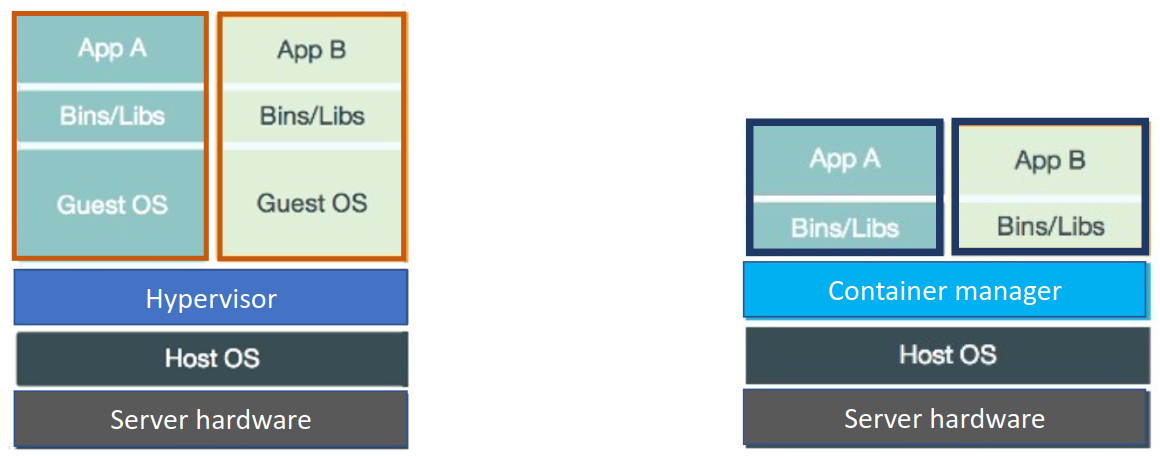
\includegraphics[width=0.8\textwidth]{images/Cloud/virtualizedresources.png}
    \caption{Virtual Machines and Containers}
    \label{fig:virtualizedresources}
\end{figure}

\subsection{Docker}

Portability of applications has been one of the biggest problems in software engineering: traditionally, there was one environment for developing and testing and another for production and distribution (the environment where the application was deployed and distributed to the user). These two environments were not the same, which meant that more time and money were required each time an application was moved between different environments.

\textbf{Docker} is a platform that allows us to run applications in an isolated environment. Docker enables the development and running of portable applications by utilizing containers: once an application is developed, it is encapsulated inside a container. When the container is opened in a new environment, it will not have portability issues, thanks to \textbf{Docker Engine} (used for creating and running containers). The \emph{Docker platform} also contains \textbf{Docker Hub}, which is used for distributing containers.

\begin{figure}[H]
    \centering
    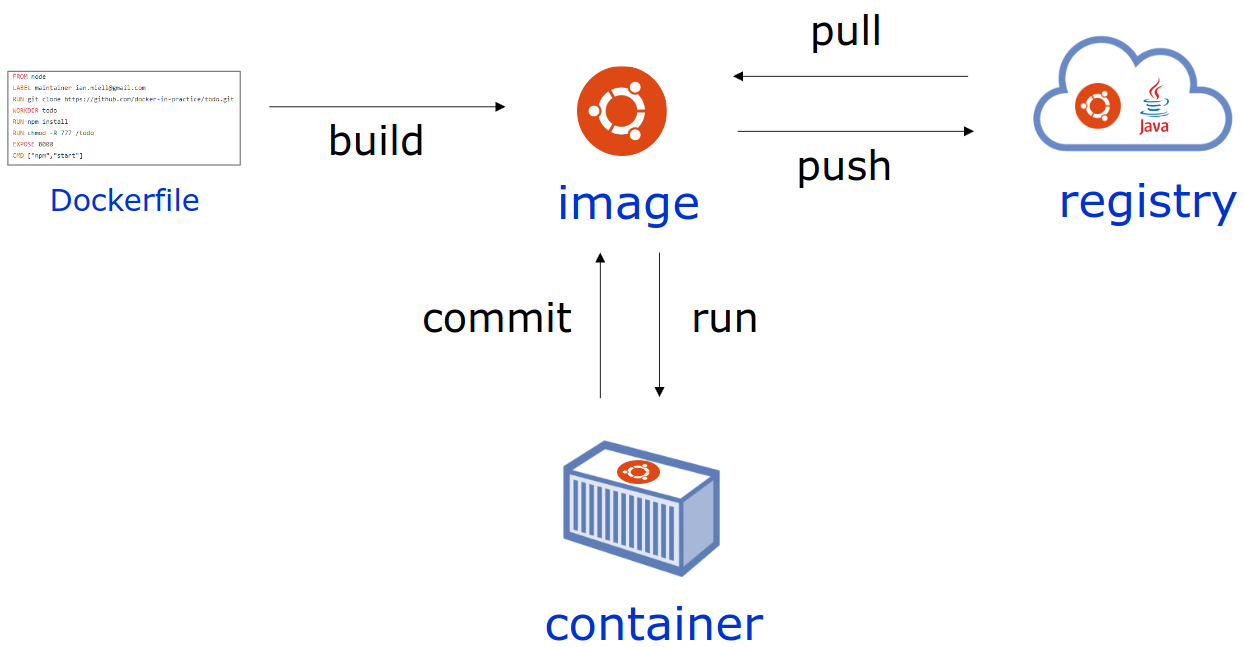
\includegraphics[width=0.8\textwidth]{images/Cloud/DockerCycle.png}
    \caption{Docker Life Cycle}
    \label{fig:DockerCycle}
\end{figure}

Software components are packaged into \textbf{images}, which are utilized as read-only templates to create and run \textbf{containers}. Since the templates are read-only, \emph{external volumes} are required to ensure data persistence. The images are stored in a (private or public) \textbf{Docker registry}: a registry structured in repositories, where each repository contains a set of images for different versions of software (images are identified by pairs repository:tag). Images are structured into layers, where each layer is in turn an image (the lowest layer is called the base image). \\

As we can see from Figure \ref{fig:DockerCycle}, the command \textbf{pull} retrieves an image from the \emph{registry}, while \textbf{push} uploads an image to the \emph{registry}. Images can be built from a \emph{Dockerfile} (see the documentation\footnote{\url{https://docs.docker.com/engine/reference/builder/}}) using the command \textbf{build}. Images can also be run in a \emph{container} using the command \textbf{run}. To modify the \emph{application} (and save a new version), the command \textbf{commit} must be used. \\

When an image generates multiple processes inside a container, the life of the container will be associated with the main process. It is good practice to create one container per process, so when the life of a process ends, it will not affect the other processes. In cases where the application consists of multiple services, Docker provides a tool called \textbf{Docker Compose} (see the documentation\footnote{\url{https://docs.docker.com/compose/}}), which not only allows running one container per service but also manages networking (it is possible to call the locally hosted services using their names) and communication between containers.

\section{Everything as a Service}

There are different deployment models of cloud computing:
\begin{itemize}
    \item \textbf{IaaS}: IaaS provides (virtualized) servers, storage, and networking. The IaaS provider manages all infrastructure. The client is responsible for all other aspects of the deployment (e.g., OS, application). Some examples include EC2 and S3.
    \item \textbf{PaaS} (Platform as a Service): PaaS provides a complete platform as a service (VMs, OS, services, SDKs, etc.). The PaaS provider manages infrastructure, OS, and enabling software. The client is responsible for installing and managing the application. Some examples include Heroku, Azure, and GAE.
    \item \textbf{SaaS} (Software as a Service): SaaS provides software on demand for use, accessible via thin clients or APIs. The SaaS provider manages infrastructure, OS, and application. The client is responsible for nothing, which is why this is the service with the largest market share. An example is Salesforce.com.
\end{itemize}

The following Figure \ref{fig:PizzaAsAService} represents an analogy of what each deployment model provides, and what clients need to manage on their own.

\begin{figure}[H]
    \centering
    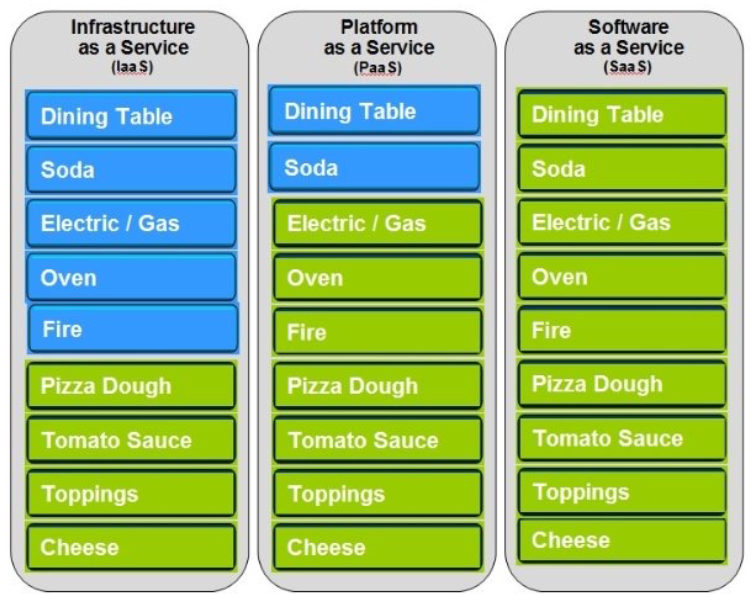
\includegraphics[width=0.8\textwidth]{images/Cloud/PizzaAsAService.png}
    \caption{Pizza as a Service}
    \label{fig:PizzaAsAService}
\end{figure}

\subsection{SaaS}

Before SaaS (\textit{Software as a Service}), software products were initially installed on customers’ computers. Customers had to configure the software and manage software updates, while software product companies had to maintain different product versions. With SaaS, the product is delivered as a service, allowing customers to avoid installation; instead, they pay a subscription and access the product remotely.\\

\noindent
Some benefits of SaaS are:
\begin{itemize}
    \item \textbf{Cash flow}: There is a regular cash flow, which means that customers pay periodic subscriptions or pay-per-use.
    \item \textbf{Update management}: The client controls product updates, so customers receive updates simultaneously. This eliminates the need to maintain multiple versions, resulting in reduced costs.
    \item \textbf{Continuous deployment}: The client can deploy new software versions as soon as changes have been made and tested.
    \item \textbf{Payment flexibility}: Different payment options can attract a wider range of customers (e.g., small companies or individuals can avoid paying large upfront software costs).
    \item \textbf{Try before you buy}: The client can make an early free or low-cost product available to gather customer feedback (e.g., a product free for a few weeks to collect feedback).
    \item \textbf{Data collection}: The client can easily collect data on product usage and customer interactions.
\end{itemize}

\noindent
Some cons of SaaS are:
\begin{itemize}
    \item \textbf{Privacy regulation compliance}: Different countries have varying strict laws regarding the storage of personal information.
    \item \textbf{Security concerns}: Customers may be hesitant to relinquish data control to an external provider, but this data needs to be managed by the SaaS provider. What happens when the SaaS provider experiences a data breach? Will they notify the clients?
    \item \textbf{Network constraints}: These can limit response times during heavy data transfers.
    \item \textbf{Data exchange}: If the cloud does not provide suitable APIs, exchanging data can be difficult. This is contract-based: depending on the offering, you might have access to different sets of data.
    \item \textbf{Loss of control over updates}: This freedom of updates can lead to excessive changes (e.g., new functionalities added daily, impacting the user interface).
    \item \textbf{Service lock-in}: It can be challenging to move code from one SaaS provider to another.
\end{itemize}

\noindent
After deciding that SaaS will be the deployment model, several design issues must be addressed:

\begin{itemize}
    \item \textbf{Local or remote processing}: Some features can be executed locally, which reduces network traffic and increases response speed but may also increase power consumption for battery-powered devices.
    \item \textbf{Authentication}: There are usually three kinds of authentication: the product’s own authentication system, federated authentication (based on mutual trust relationships between a Service Provider (SP) such as an application vendor and an external Identity Provider (IdP)), and individual credentials (e.g., Google, LinkedIn).
    \item \textbf{Information leakage}: If the service is offered to multiple organizations, there's a security risk when a member of one organization handles data belonging to another.
    \item \textbf{Multi-tenant or multi-instance database management}: Multi-tenant systems use a single repository (with advanced techniques to partition data and control those partitions), while multi-instance systems have separate copies of the system and database.
\end{itemize}

\subsection{Multi-tenant and Multi-instance Systems}

\subsubsection{Multi-tenant Systems}
\textit{Multi-tenant systems} use a single database schema shared by all system users. The items in the database are tagged with a tenant identifier to provide “logical isolation,” meaning that users will only be able to access data linked to their tenant, as shown in Figure \ref{fig:multi-tenant-example}.

\begin{figure}[H]
    \centering
    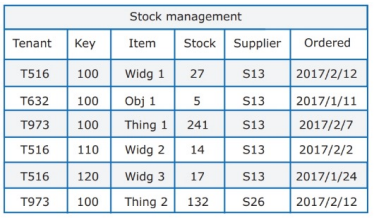
\includegraphics[width=0.6\textwidth]{images/Cloud/multi-tenant-example.PNG}
    \caption{Multi-tenant database schema example}
    \label{fig:multi-tenant-example}
\end{figure}

\noindent
Some advantages of a \textit{multi-tenant system} are:
\begin{itemize}
    \item \textbf{Resource utilization}: The SaaS provider has control over all resources used by the software and can optimize it to make effective use of these resources.
    \item \textbf{Security}: Multi-tenant databases must be designed for security since data for all customers are stored in the same database. They are, therefore, likely to have fewer security vulnerabilities than standard database products. Security management is also simplified as there is only a single copy of the database software to patch if a security vulnerability is discovered.
    \item \textbf{Update management}: It is easier to update a single instance of software rather than multiple instances. Updates are delivered to all customers simultaneously, ensuring that everyone uses the latest version.
\end{itemize}

\noindent
However, there are also challenges associated with a \textit{multi-tenant system}:
\begin{itemize}
    \item \textbf{Inflexibility}: Customers must all use the same database schema, with limited scope for adapting this schema to individual needs.
    \item \textbf{Security}: Since data for all customers is maintained in the same database, there is a theoretical risk of data leaking from one customer to another. More seriously, if there is a database security breach, it can affect all customers.
    \item \textbf{Complexity}: Multi-tenant systems are usually more complex than multi-instance systems due to the need to manage many users, which increases the likelihood of bugs in the database software.
\end{itemize}

Mid-size and large businesses rarely want to use generic multi-tenant software; they often prefer a \textbf{customized version} adapted to their own requirements. One solution is to add extra fields to each table and allow customers to use these fields as they wish. However, predicting how many extra columns to include is challenging (too few will be insufficient, and too many will lead to wasted space), and different customers are likely to need different types of columns. A second solution is to add a field to each table that identifies a separate “extension table,” allowing customers to create these extension tables to reflect their needs. This approach adds a new layer of complexity to a system that is already complex.

\textbf{Security} is the major concern for corporate customers using multi-tenant databases. Since information from all customers is stored in the same database, a software bug or attack could expose the data of some or all customers to others. To mitigate these risks, \emph{multilevel access control} (where access to data is controlled at both the organizational and individual levels) and \emph{encryption of data} (to ensure that corporate users' data cannot be viewed by people from other companies in the event of a system failure) are typically applied. Usually, only sensitive data is encrypted.

\subsubsection{Multi-instance Systems}

A \textit{multi-instance system} allows each customer to have its own system tailored to its needs, including its own database and security controls. This type of system is conceptually simpler than multi-tenant systems and avoids security concerns such as inter-organization data leakage.\\

\noindent
There are two ways to implement multi-instance systems:
\begin{itemize}
    \item \textbf{Virtual Machine-based}: Each software instance and database for a customer runs in its own Virtual Machine. This allows all users from the same customer to access the shared system database.
    \item \textbf{Container-based}: Each user has an isolated version of the software and database running in a set of containers. This solution is best suited for products where users mostly work independently with little data sharing (e.g., for individual users).
\end{itemize}
It is also possible to run containers on a virtual machine: a business could have its own VM-based system and run containers on top of this for individual users.

\newpage
\noindent
Some advantages of a \textit{multi-instance system} are:
\begin{itemize}
    \item \textbf{Flexibility}: Each instance of the system can be tailored and adapted to the customer's needs.
    \item \textbf{Security}: Each customer has its own database, so there's no possibility of data leakage from one customer to another.
    \item \textbf{Scalability}: Instances of the system can be scaled according to the needs of individual customers. For example, some customers may require more powerful servers than others.
    \item \textbf{Resilience}: If a software failure occurs, it will probably affect only a single customer, allowing other customers to continue working as normal.
\end{itemize}

\noindent
However, there are also challenges associated with a \textit{multi-instance system}:
\begin{itemize}
    \item \textbf{Cost}: It is more expensive to use multi-instance systems due to the cost of renting multiple VMs in the cloud and managing multiple systems. Since VMs have a slow startup time, they may need to be rented and kept running continuously, even if there is very little demand for the service. 
    \item \textbf{Update management}: Managing updates for many instances can be complex, especially if the instances have been tailored to specific customer needs.
\end{itemize}

\section{Cloud Software Architecture}

During the initial stages of designing a cloud software architecture, several \textbf{architectural decisions} must be made: Should the software use a multi-tenant or multi-instance database? (\emph{Database organization}) What are the software scalability and resilience requirements? (\emph{Scalability and resilience}) Should the software structure be monolithic or service-oriented? (\emph{Software structure}) The answers to these questions will guide the decision regarding which cloud platform should be used for deployment and delivery.

\subsection{Database Organization}

There are three possible ways to provide a customer database in a cloud-based system:
\begin{enumerate}
    \item As a \textit{multi-tenant system}, shared by all customers of your product. This may be hosted in the cloud using large, powerful servers.
    \item As a \textit{multi-instance system}, with each customer database running on its own virtual machine.
    \item As a \textit{multi-instance system}, with each database running in its own container. The customer database may be distributed across several containers.
\end{enumerate}
\newpage
\noindent
Some factors that can help decide the appropriate method for providing a customer database in a cloud-based system include:
\begin{itemize}
    \item \emph{Target customers}: Do customers require different database schemas and personalization? If so, use a multi-instance database.
    \item \emph{Transaction requirements}: Is it critical that the product supports ACID transactions, ensuring that data is consistently accurate at all times? If so, consider a multi-tenant database or a VM-based multi-instance database.
    \item \emph{Database size and connectivity}: How large is the typical database used by customers? How many relationships exist between database items? A multi-tenant model is usually best for very large databases, as it allows you to focus efforts on optimizing performance.
    \item \emph{Database interoperability}: Will customers wish to transfer information from existing databases? What are the differences in schemas between these and a possible multi-tenant database? What software support will they expect for the data transfer? If customers have many different schemas, a multi-instance database should be used.
    \item \emph{System structure}: Are the developers using a service-oriented architecture for the system? Can the customer database be split into a set of individual service databases? If so, use a containerized multi-instance database.
\end{itemize}

\subsection{Scalability and Resilience}

\subsubsection{Scalability}

Scalability (the ability to adapt automatically to load changes) can be achieved by adding new virtual servers (\textbf{scaling out}) or by increasing the power of an existing server (\textbf{scaling up}) in response to increasing load. Scaling out is typical of cloud-based systems: the product must be organized so that individual software components can be replicated and run in parallel, while load-balancing mechanisms direct requests to different instances of the components (e.g., using PaaS).

\subsubsection{Resilience}

Resilience (the ability to continue delivering critical services in the event of system failure or malicious activity) is realized using a technique known as \textbf{hot standby}, which involves maintaining replicas of software and data in different locations (see Figure \ref{fig:hot-standby}). Database updates are mirrored, and a system monitor continuously checks system status. A cheaper alternative is called \textbf{cool standby}, where, in the event of system failure, the data is restored from a backup (meaning the system will be unavailable until the data restoration is complete).

\begin{figure}[H]
    \centering
    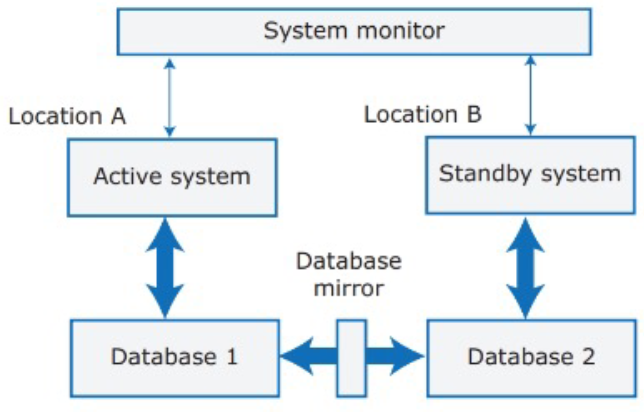
\includegraphics[width=0.6\textwidth]{images/Cloud/hot-standby.png}
    \caption{Hot standby technique schema}
    \label{fig:hot-standby}
\end{figure}

\subsection{Software Structure}

The main choice here is between \textbf{monolithic systems} or \textbf{fine-grained, stateless services}. The latter uses independent services that can be replicated, distributed, and migrated. This approach is particularly suitable for cloud-based software with services deployed in containers. The monolithic approach is often employed to build prototypes, especially if a fine-grained system better fits the specific situation.\\

\noindent
When choosing a cloud platform, there are two main points to consider:

\begin{enumerate}
    \item \textbf{Technical issues}: \emph{Expected load and load predictability}, \emph{resilience}, \emph{supported cloud services} (which cloud services a provider can offer), and \emph{privacy and data protection} (some EU countries have strict requirements regarding data protection and storage locations $\rightarrow$ necessitating cloud providers to offer guarantees on storage locations).
    \item \textbf{Business issues}: \emph{Developer experience} (the languages and technologies depend on the team's experience), \emph{Service-level agreements} (guarantees provided by the cloud provider), \emph{Portability and cloud migration} (to create an ``exit plan'' to mitigate vendor lock-in), \emph{target customers} (customers may have older systems that need to interoperate with the new ones), and \emph{cost} (including all developer and technology-related expenses).
\end{enumerate}

\section{Container Orchestration}

As mentioned in the previous section, containers provide a lightweight mechanism for isolating an application's environment. Container images can be executed reliably on any machine, offering portability (we used Docker) from development to deployment. 

\newpage
\noindent
\textbf{Automated deployment}, such as that provided by Docker, often has limited capability for optimizing memory usage and may not utilize resources effectively. Additional concerns arise: What happens if your container dies? What happens if the machine running your container fails? What if you have multiple containers that need to communicate with one another (\emph{inter-node communication})? How do you enable networking between containers? If your production environment consists of multiple machines, how do you decide which machine to use to run your container?

The solution comes with \textbf{container orchestration}: the architect of a system defines the containers to be run and then hands over control to the \emph{container orchestration platform} to realize that vision.

\subsection{Kubernetes}

One of the most used container orchestration platforms is \textbf{Kubernetes}, which manages the entire lifecycle of individual containers, spinning up and shutting down resources as needed (if a container shuts down unexpectedly, K8s reacts by launching another container in its place). K8s provides a mechanism for applications to communicate with each other even as the underlying individual containers are created and destroyed. Given a set of container workloads to run and a set of machines in a cluster, the container orchestrator examines each container and determines the optimal machine to schedule that workload.

Kubernetes will ingest through its API a ``\emph{Desired State Management},'' which is a YAML manifest. The manifest specifies, given a set of images, which are the \textbf{Pods} (groups of images). Kubernetes will insert inside the same node all the images that are defined in the same Pod, generating as many replicas as defined. A node can handle multiple Pods. If one of the nodes (worker = container host) fails, Kubernetes detects the broken node and starts a new replica, as shown in Figure \ref{fig:K8s5mins}. The \emph{Kubernetes cluster services} not only handle that but also handle communication between the nodes (the existing ones and the ones that will be created).

\begin{figure} [H]
    \centering
    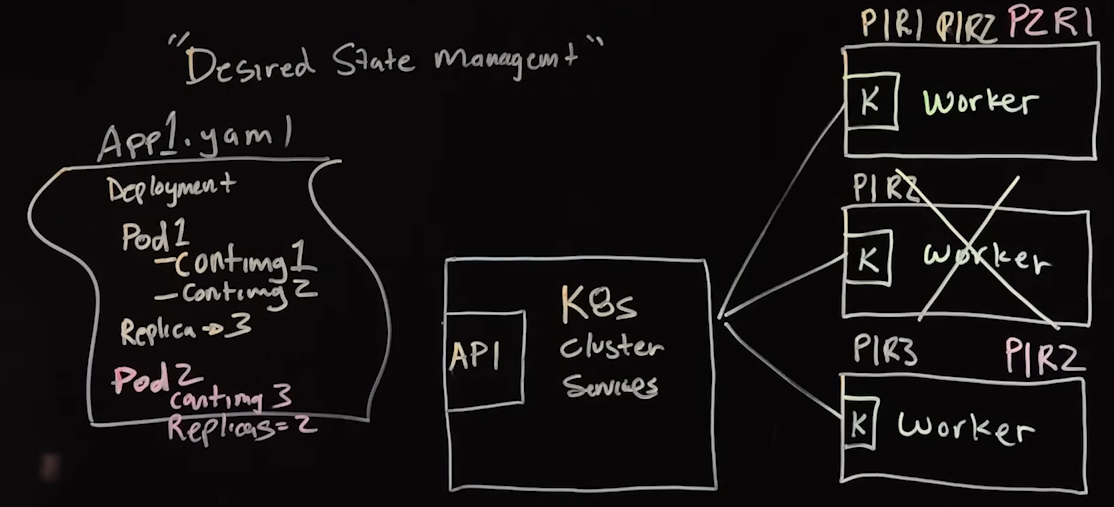
\includegraphics[width=0.8\textwidth]{images/Cloud/K8s5mins.png}
    \caption{Kubernetes' management idea}
    \label{fig:K8s5mins}
\end{figure}

\subsection{Kubernetes Design Principles}

Here are the design principles of Kubernetes:
\begin{itemize}
    \item \textbf{Declarativeness}: A declarative approach is to simply define the desired state of a system (with the manifest). K8s will detect when the actual state of the system doesn't meet our expectations and will intervene to fix the problem, making our system self-healing. The desired state is defined by a collection of objects: each object has a specification in which you provide the desired state and a status that reflects the current state of the object. K8s constantly polls each object to ensure that its status is equal to the specification: if an object is unresponsive, K8s will spin up a new version to replace it; while if an object's status has drifted from the specification, K8s will issue the necessary commands to drive that object back to its desired state.
    \item \textbf{Distribution}: Kubernetes provides a single unified interface for interacting with a cluster of machines. In this way, developers don't have to worry about communicating with each machine individually.
    \begin{figure} [H]
        \centering
        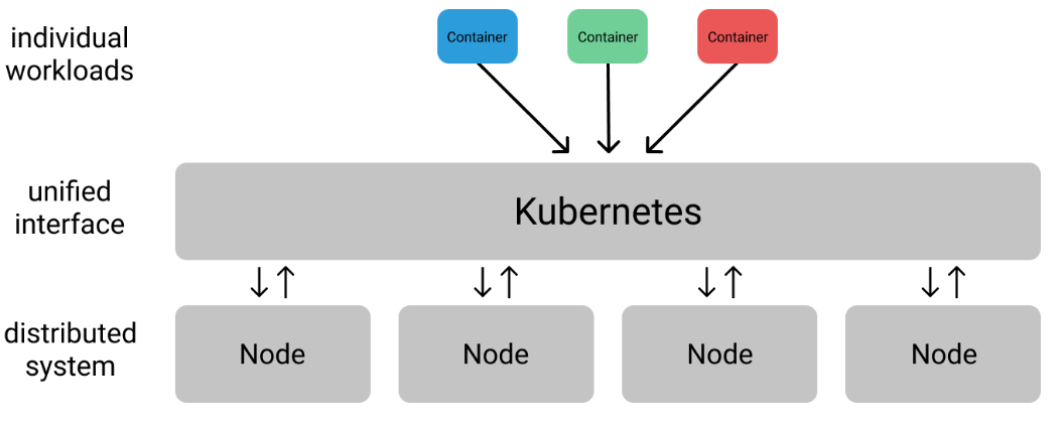
\includegraphics[width=0.75\textwidth]{images/Cloud/K8sDistribution.png}
        \caption{Kubernetes distribution schema}
        \label{fig:K8sDistribution}
    \end{figure}
    \item \textbf{Decoupling}: Containers should be developed with a single concern in mind: microservice-based architecture. K8s naturally supports the idea of decoupled services that can be scaled and updated independently.
    \item \textbf{Immutable infrastructure}: To get the most from containers and container orchestration, an immutable infrastructure should be deployed. This means that instead of logging into a container on a machine to update a library, it is required to build a new container image, deploy the new version, and terminate the older version. The reason is that containers are designed to be ephemeral, ready to be replaced by another container instance at any time. Maintaining immutable infrastructure makes it easier to roll back applications to a previous state (e.g., if an error occurs) by simply updating the configuration to use an older container image.
\end{itemize} 

\subsection{Kubernetes objects}

There are many objects defined by Kubernetes that can be specified in the \textbf{manifests} (either in JSON or YAML). Here's a list of the main ones:
\begin{itemize}
    \item \textbf{Pod}: The minimum Kubernetes deployment unit, which is composed of one or more (tightly related) containers, a shared networking layer, and shared filesystem volumes. Pods can't be distributed by themselves. Each Pod is assigned a unique IP address that we can use to communicate with it.
    \begin{figure} [H]
        \centering
        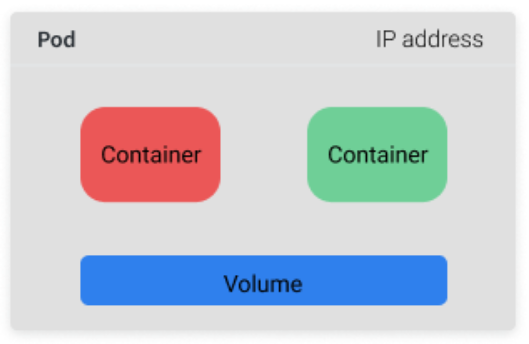
\includegraphics[width=0.6\textwidth]{images/Cloud/K8sPod.png}
        \caption{Kubernetes Pod schema}
        \label{fig:K8sPod}
    \end{figure}
    \item \textbf{Deployment}: It includes a collection of Pods defined by a template and a replica count (number \(n\) of how many copies of the template we want to run). The cluster will always try to have \(n\) Pods available.
    \begin{figure} [H]
        \centering
        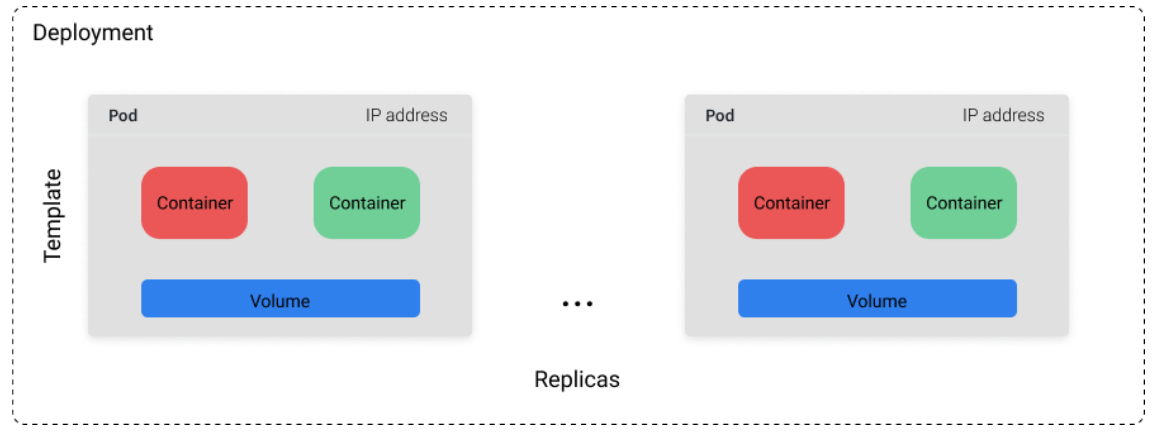
\includegraphics[width=1\textwidth]{images/Cloud/K8sDeployment.png}
        \caption{Kubernetes Deployment schema}
        \label{fig:K8sReplica}
    \end{figure}
    \newpage
    \item \textbf{Service}: The Service object provides a stable endpoint to direct traffic to the desired Pods even as the exact underlying Pods change due to updates/scaling/failures. Services know which Pods they should send traffic to (even if the set of Pods running as part of the Deployment can change at any time) based on labels (key-value pairs) that we define in the Pod metadata.
    \begin{figure} [H]
        \centering
        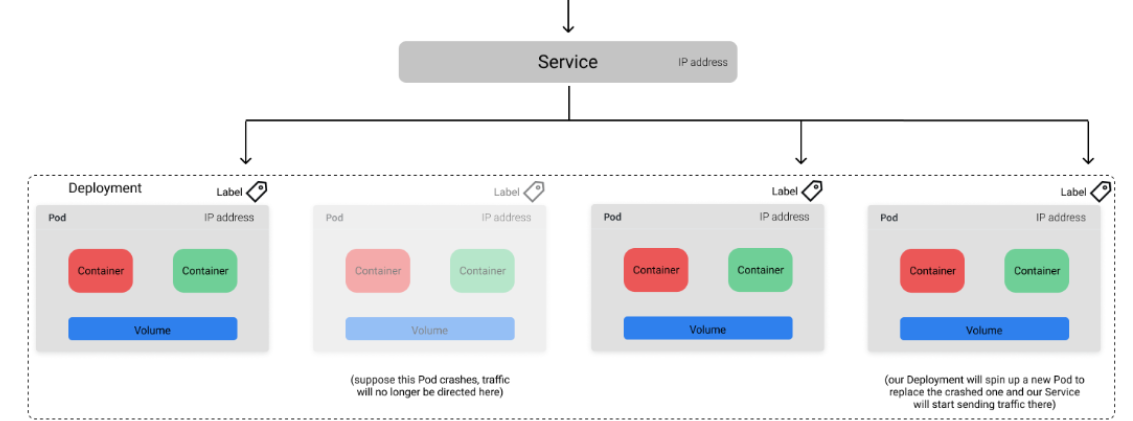
\includegraphics[width=1\textwidth]{images/Cloud/K8sService.png}
        \caption{Kubernetes Service schema}
        \label{fig:K8sService}
    \end{figure}
	\item \textbf{Ingress}: To expose the application to traffic external to the cluster, it is necessary to define an Ingress object. It is possible to select which Services to make publicly available and expose applications behind a stable endpoint (only available to internal cluster traffic).
     \begin{figure} [H]
        \centering
        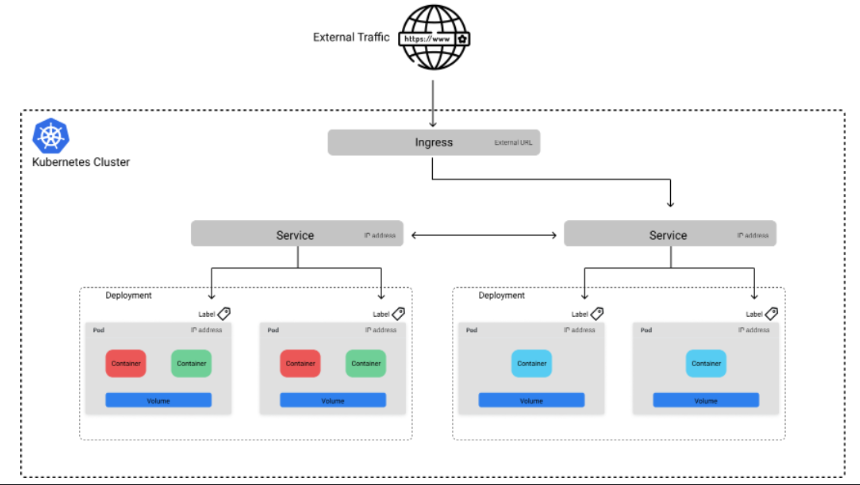
\includegraphics[width=1\textwidth]{images/Cloud/K8sIngress.png}
        \caption{Kubernetes Ingress schema}
        \label{fig:K8sIngress}
    \end{figure}
\end{itemize}

\subsection{Kubernetes control plane}

In this subsection, a high-level description of how Kubernetes works underneath will be provided. There are two types of machines in a cluster (set of machines): the \textbf{master node} (often single), which is a machine that contains most of the control plane components, and the \textbf{worker nodes}, which are machines that run the application workloads.

\subsubsection{Master node}

Users provide new/updated object specifications (manifests) to the API server of the master node. The \textbf{API server} validates update requests (with some input verification) and acts as a unified interface for questions about the cluster's current state. The \emph{state of the cluster} (cluster configuration, object specifications, object statuses, nodes in the cluster, object-node assignments, etc.) is stored in a distributed key-value store named \textit{etcd}.

The Master node (as shown in Figure \ref{fig:K8sMaster}) is composed of the \emph{API Server}, the distributed key-value store \textbf{etcd} (which contains the entire state of the cluster), a \emph{controller-manager}, and a \emph{scheduler}. The reason why the API server works as an intermediary is to reinforce the decoupling principle: each of these components is responsible for only one task (which also makes failure recovery easier).\\

The \textbf{controller-manager} monitors the cluster state through the API server. If the actual state differs from the desired state, the controller-manager will make changes via the API server to drive the cluster towards the desired state.

\begin{figure} [H]
    \centering
    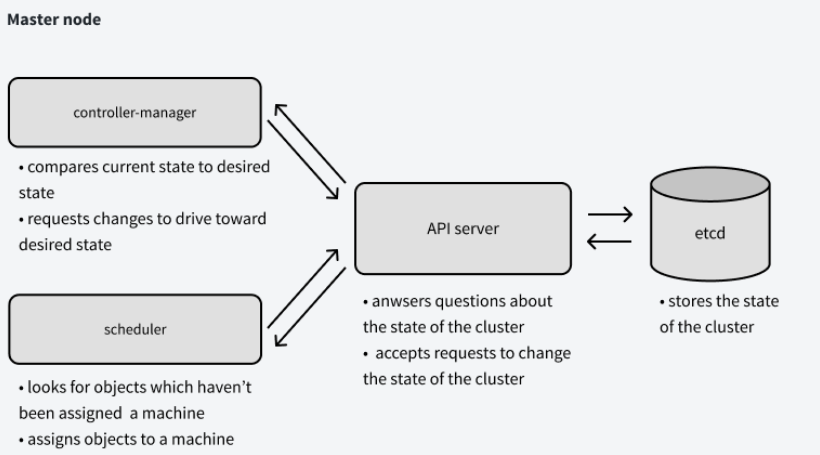
\includegraphics[width=1\textwidth]{images/Cloud/K8sMaster.png}
    \caption{Kubernetes Master node structure}
    \label{fig:K8sMaster}
\end{figure}
\newpage
The \textbf{scheduler} decides where objects should be run, as shown in the below Figure \ref{fig:K8sMasterScheduler}. The scheduler asks the API server which objects haven't been assigned to a machine (1), determines which machines those objects should be assigned to (2), and then replies back to the API server (3) to reflect this assignment (4).

\begin{figure} [H]
    \centering
    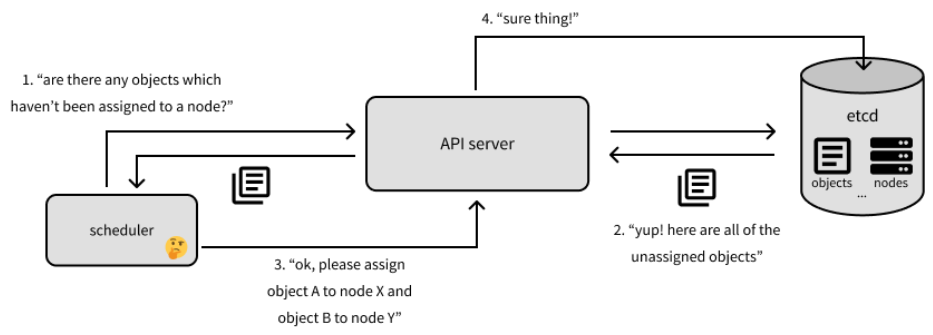
\includegraphics[width=1\textwidth]{images/Cloud/K8sMasterScheduler.png}
    \caption{Scheduler life-cycle}
    \label{fig:K8sMasterScheduler}
\end{figure}

\subsubsection{Worker node}

Every worker node contains a \textbf{kubelet}, which acts as the node's ``agent'' that communicates with the API server to see which container workloads have been assigned to the node. It is responsible for spinning up pods to run these assigned workloads. When a node first joins the cluster, the kubelet announces the node's existence to the API server so the scheduler can assign pods to it.
Workers also contain \textbf{kube-proxy}, which enables containers to communicate with each other across the various nodes in the cluster. With Figure \ref{fig:K8sStructure}, it is possible to observe the entire Kubernetes structure.

\begin{figure} [H]
    \centering
    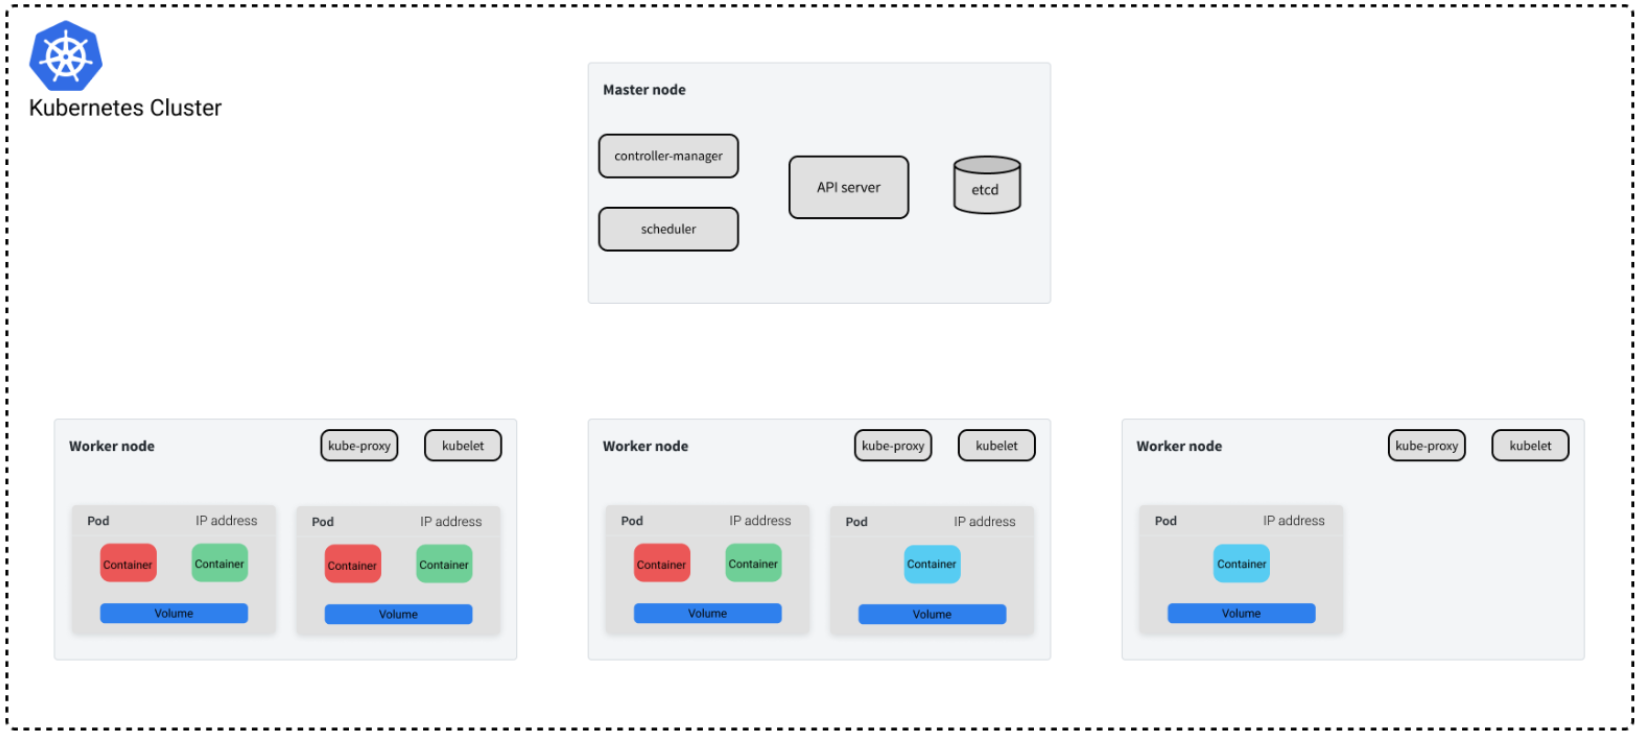
\includegraphics[width=1\textwidth]{images/Cloud/K8sStructure.png}
    \caption{Kubernetes entire structure}
    \label{fig:K8sStructure}
\end{figure}

To conclude this chapter, in which cases is the use of Kubernetes not the best choice?
\begin{itemize}
    \item If you can run your workload on a single machine.
    \item If your compute needs are light.
    \item If you don't need high availability and can tolerate downtime.
    \item If you don't envision making a lot of changes to your deployed services.
    \item If you have a monolith and don't plan to break it into microservices.
\end{itemize}

There's also a way to do container orchestration with Docker (it's called \emph{Docker Swarm}), but Kubernetes is a much stronger orchestrator. Still, they have a partnership, so there's no lock-in between Docker and Kubernetes.
